\chapter{反激式开关电源变换器工作机制}
本章研究开关电源的工作机制,首先阐述反激式开关电源的拓扑结构,然后分析反激式开关电源的各种工作模式、脉宽调制方式、不同的环路控制方式和两种反馈方式。为后续完成芯片工作流程与功能模块的构建,根据芯片应用电路和功 能对系统的外围器件和内部参数指标进行设计。

\section{拓扑结构分析}
反激式 AC/DC 变换器的主要功能为将从交流电整流得到的直流高压转化为目标 负载所需要的输出电压。主要适用于中小功率的应用场景,其本身由 Buck-boost 拓扑衍生而来,考虑到对电路安全性要求较高,在常规的 buck-boost 结构中加入变压器取代电感线圈发展出电气隔离结构,即隔离型反激式变换器。
\subsection{传统反激式拓扑结构}

\subsection{准谐振反激式拓扑结构}
                

\subsection{非对称半桥反激式拓扑结构}

\section{开关电源的工作模式}
\label{sec:dataset-build}
\subsection{CCM连续导通模式}
对于非对称半桥反激式开关电源变换器而言,不同于传统的反激式开关电源变换器,连续导通模式是指,当系统给出功率开关管的下一周期导通信号时,变压器原边电感电流和励磁电感电流未重合,变压器励磁电感中的能量还没有完全退磁转移到次级侧负载,紧接着又从输入端开始继续获取能量。

非对称半桥反激式开关电源变换器在连续导通模式下的波形如下图所示,tHSon是高边功率管HS的导通时间,tLSon是低边功率管LS的导通时间,Vhb是高低边功率管的中间节点电压,VCr是初级侧谐振电容的两端电压差,Ihb是初级侧电感电流,ILm是励磁电感电流,Isec是次级侧电感电流。

当高边功率管导通时,输入电压的能量在变压器励磁电感和谐振电容中积累,当高边功率管关断时,励磁电感和谐振电容中的能量经由副边绕组传递到输出端。当下一周期高边功率管导通再次开始励磁时,变压器励磁电感和谐振电容中储存的能量还未完全退磁传递到副边绕组的工作模式就是CCM模式。

在输入输出电压稳定运行期间,对励磁电感应用伏秒平衡原理,能够得到输入电压、输出电压和占空比D之间的关系。在tHSon内,励磁电感两端电压为输入电压减去谐振电容电压Vcr;在tLSon内,励磁电感两端电压为谐振电容电压Vcr,由此可得式\eqref{eq:CCM_1}:

\begin{equation}
    \label{eq:CCM_1}
    D\times(V_{in}−V_{cr\_avg})=(1−D)\times V_{cr\_avg}
\end{equation}

\begin{equation}
    \label{eq:Vcr_1}
    V_{cr\_avg}=N \times V_o\times\frac{L_m}{L_m+L_r}
\end{equation}
其中$V_{cr\_avg}$是谐振电容Cr上的平均电压,它等于输出电压经变压器原边励磁电感和漏感分压后乘以匝数比N。

对式\eqref{eq:CCM_1}和\eqref{eq:Vcr_1}进行整理可得式\eqref{eq:CCM_3}:

\begin{equation}
    \label{eq:CCM_3}
    V_o=D \times \frac{V_{in}}{N} \times\frac{L_m}{L_m+L_r}  
\end{equation}

根据式\eqref{eq:CCM_3}可知输出电压由占空比D、输入电压、变压器匝数比N、变压器励磁电感和漏感决定,与负载恒和频率无关。由于Lr对Lm而言非常小可以忽略不计,式\eqref{eq:CCM_3}可化简为式\eqref{eq:CCM_4}:

\begin{equation}
    \label{eq:CCM_4}
    V_o=D \times \frac{V_{in}}{N}  
\end{equation}

\subsection{DCM断续导通模式}




\subsection{CRM临界导通模式}


\section{工作原理}

针对\eqref{subsec:MR-PPFN Adaptive Feature Fusion Network Design Problem Analysis}提出的问题,本小节提出一种自适应特征融合网络,结构如图\eqref{fig:Adaptive Fusion NetWork}所示,网络的输入分别是点云特征$P$和目标特征$T$,为了方便融合这两种特征,首先分别通过线性层进行将特征映射到相同的维度,而且为了适应不同点云子网络学习的点云特征的差异性,采取拼接、乘性、注意力三种融合方式进行加权融合,并且加权的参数是可学习的,从而可以更加有效地融合MR-PPFN并行网络学习到的点云与目标点特征。 

在三种融合策略中,注意力机制是通过计算输入特征之间的相关性来动态地调整特征的重要程度,突出关键特征,抑制不相关或冗余的信息。在特征融合中,注意力机制可以帮助模型专注于输入特征中最有用的部分,从而提高特征表示的质量。
而特征连接是通过将不同来源的特征直接拼接在一起,从而保留了所有输入特征的信息。这种方法简单且有效,可以为后续的网络层提供丰富的特征信息。
乘性融合是通过逐元素地相乘两个特征,强调它们之间的交互关系,这种方法可以捕捉到特征之间的非线性关系。

假设输入的点云特征向量为 \( P \in \mathbb{R}^{n \times d_p} \),目标特征向量为 \( T \in \mathbb{R}^{n \times d_t} \)。
首先,将点云特征和目标特征投影到一个共同的特征空间:
\begin{equation}
    P' = W_p P + b_p
\end{equation}
\begin{equation}
    T' = W_t T + b_t
\end{equation}
其中,\( W_p \in \mathbb{R}^{d_f \times d_p} \) 和 \( W_t \in \mathbb{R}^{d_f \times d_t} \) 是投影矩阵,\( b_p \in \mathbb{R}^{d_f} \) 和 \( b_t \in \mathbb{R}^{d_f} \) 是偏置向量。

其次是通过公式\eqref{eq:attention}计算注意力权重,其中的\( W_q, W_k \in \mathbb{R}^{d_f \times d_f} \) 是注意力机制的权重矩阵。
\begin{equation}
    \label{eq:attention}
    A = \text{softmax}\left(\frac{(P' W_q) (T' W_k)^T}{\sqrt{d_f}}\right)
\end{equation}

紧接着结合拼接、乘性、注意力三种融合策略:
\begin{align}
    F_{\text{attention}} &= A (T' W_v) \\
    F_{\text{concat}} &= \text{ReLU}(W_c [P'; T']) \\
    F_{\text{mul}} &= \text{ReLU}(P' \odot T')
\end{align}
其中,\( W_v \in \mathbb{R}^{d_f \times d_f} \) 是用于计算输出特征的权重矩阵,\( W_c \) 是用于连接特征的权重矩阵。

最后通过可学习的权重进 \(\alpha, \beta, \gamma\)行加权求和,如公式\eqref{eq:calculate fusion feature}所示,并且权重参数之间满足 \(\alpha + \beta + \gamma = 1\),得到最终的融合特征$F$。
\begin{equation}
    \label{eq:calculate fusion feature}
    F = \alpha F_{\text{attention}} + \beta F_{\text{concat}} + \gamma F_{\text{mul}}
\end{equation}



\begin{figure}[htbp] 
    \centering
    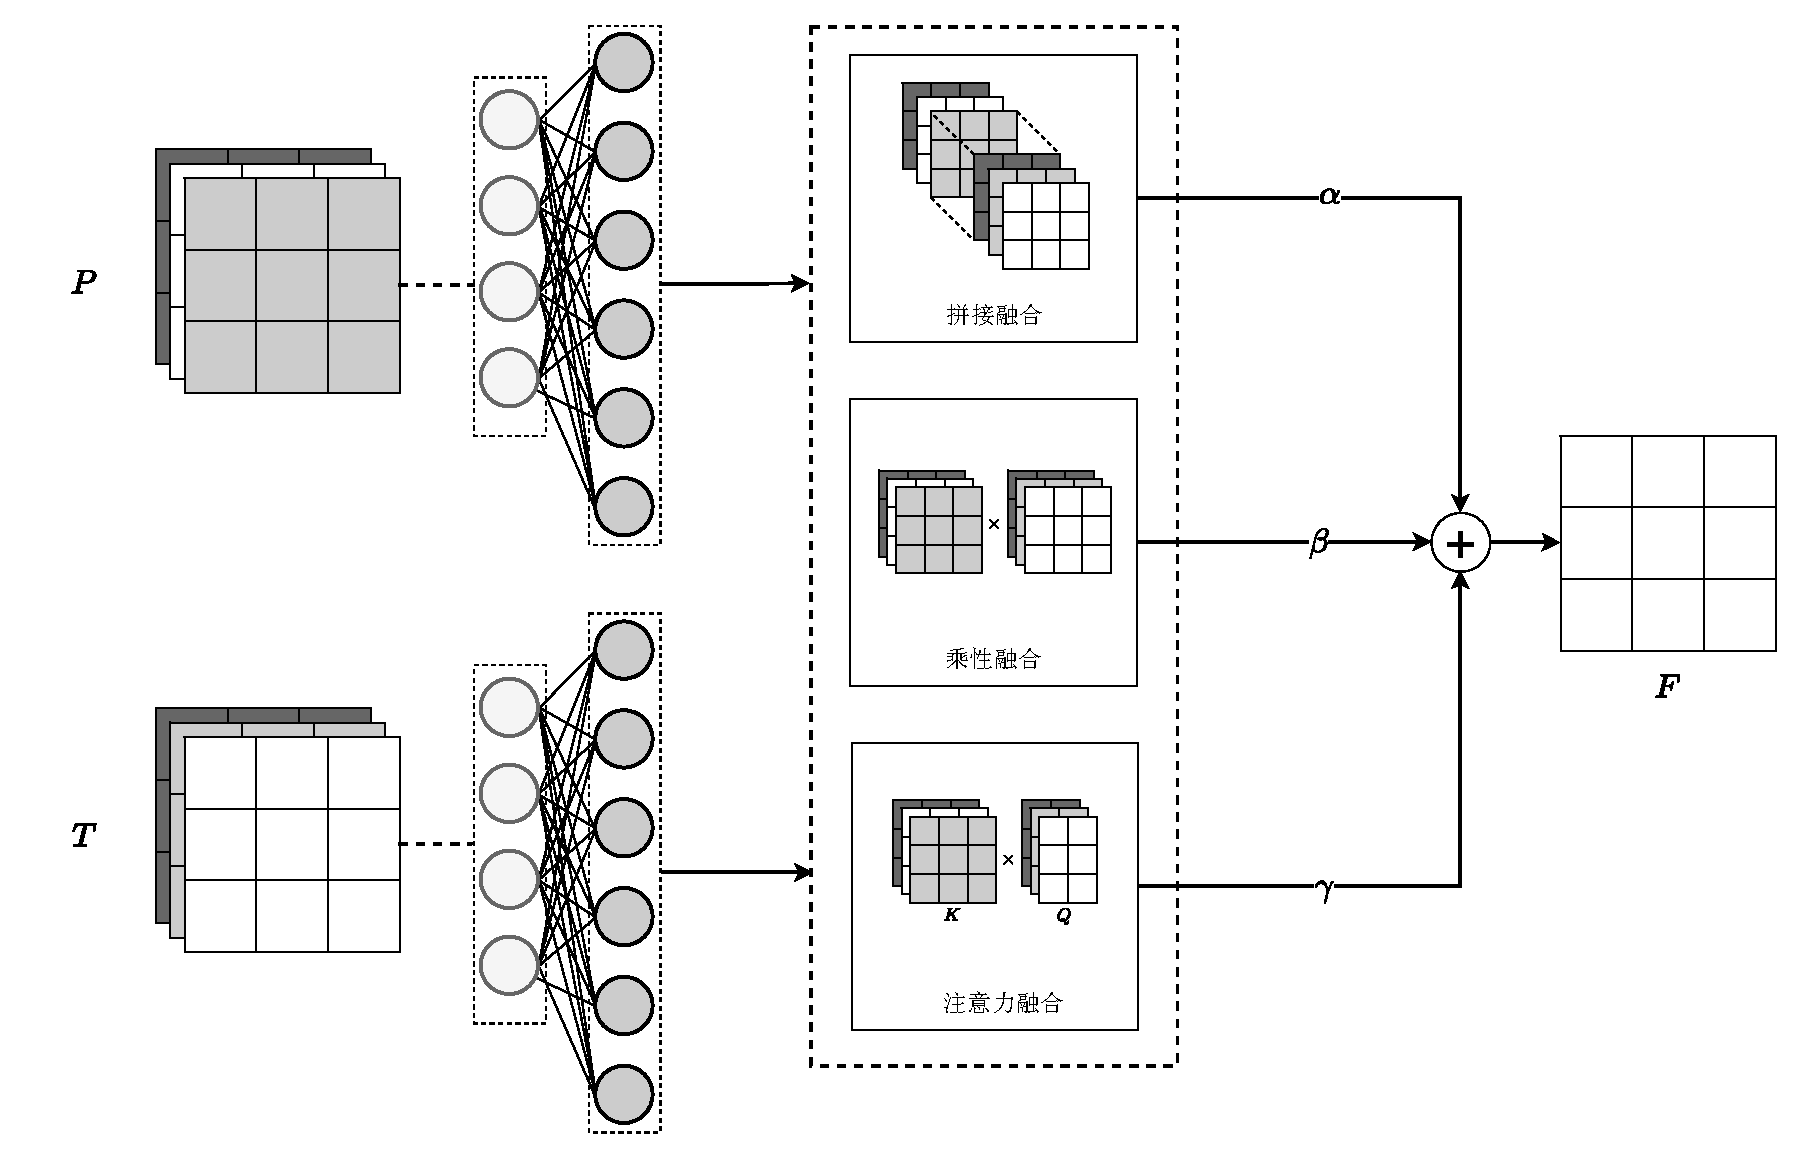
\includegraphics[width=0.8\linewidth]{imgs/Adaptive Fusion NetWork.pdf}
    \caption{自适应特征融合网络}
    \label{fig:Adaptive Fusion NetWork}
\end{figure}

\section{开关电源的脉宽调制方式}
开关电源通过调节开关管控制信号的导通关断时间来改变信号占空比由此达到稳定输出电压或输出电流的目的,根据改变占空比方式的不同将会得到不同的开关电源调制方式,本节将分别介绍脉冲宽度调制(PWM)、脉冲频率调制(PFM)、脉冲跳周期调制(PSM)以及脉冲宽度频率调制(PWM-PFM)。

\subsection{PWM调制方式}
PWM调制的原理是指在功率管开关频率不变的情况下通过控制功率管管的导通时间来改变占空比的大小进而维持输出电压或输出电流的稳定,即定频调宽。这是开关电源变换器中最常用的一种调制方式,常见的PWM脉宽调制系统如下图所示,是将输出电压通过电阻串进行分压后产生的输出反馈信号Vfb与参考电压在误差放大器中进行比较,产生误差放大信号Vea,Vea再与频率固定的三角波信号在PWM比较器中比较,生产占空比不同的PWM控制信号来控制功率管的导通和关断,其中电压模的锯齿波信号由固定电路给定,电流模的锯齿波信号由原边电流采样电阻上的电压处理得到。

\begin{figure}[htbp] 
    \centering
    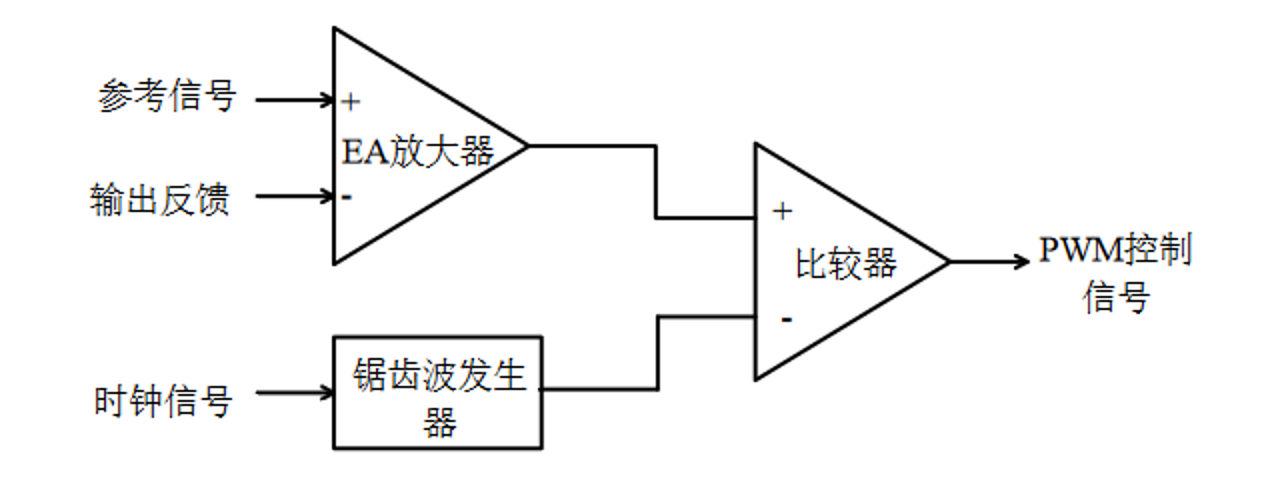
\includegraphics[width=0.8\linewidth]{figures/PWM调制1.png}
    \caption{PWM调制原理图}
    \label{fig:PWM调制1}
\end{figure}

当输出负载电流变大,输出负载会从输出电容中抽取能量,输出电压Vo变小,相应Vfb也变小,因此误差放大信号Vea增大,Vea与锯齿波信号比较后得到的脉冲宽度就会增大,导致PWM控制信号的占空比增大,将更多的能量在下一个周期中传递到副边电路维持输出电压的稳定。PWM调制作为最常用的调制方式,具有控制结构简单易于设计和实现、输出电压纹波小,动态响应快,线性度高,频率特性好等优点。但PWM调制由于频率固定,其更适用于重载情况下,因为不论输出负载大小如何,每个周期功率管都会进行导通关断操作,导致当输出负载处于空载和轻载情况下造成更多的开关损耗,电路的能量转换效率很低。

\subsection{PFM调制方式}
PFM调制的原理是指在功率管导通时间不变的情况下通过控制功率管的开关频率来改变占空比的大小进而维持输出电压或输出电流的稳定,即定宽调频。

常见的PWM脉宽调制系统如下图所示,同样是将输出电压通过电阻串进行分压后产生的输出反馈信号Vfb与参考电压在误差放大器中进行比较,产生误差放大信号Vea,不同于PWM调制,PFM调制的Vea信号输入到脉冲调制器中产生时钟信号CLK控制功率管的导通;功率管导通时长由原边电流采样电阻上的电压Vcs与给定的参考电压Vcsref比较所得的关闭信号控制。当脉冲调制器中
\subsection{PSM调制方式}
利用恒频恒宽进行调节的方式称为脉冲跳周期调制,这样一种全新的控制模式被 应用于开关功率变换器,当使用 PSM 调制时脉冲的宽度和频率保持恒定,这些脉冲 作为开关管的输入信号,所需要周期的个数会由负载的大小来进行决定。当参考电压 大于输出电压,恒定频率和宽度的时钟控制信号允许功率开关管在该周期中工作,当参考电压小于输出电压时,该周期将会被开关管忽略。PSM 调制模式其效率并不取决于输出功率,当负载发生变化时效率仍然保持恒 定,脉冲跳周期调制模式的优点是轻负载时的转换效率比脉冲宽度调制模式高、抗干扰能力强、静态功耗低;跳过一些工作周期后,会带来很大的输出电压波纹、线性调 整率变差、系统的有效频率降低等缺点。
\subsection{PWM+PFM调制方式}
PWM-PFM 是一种将 PWM 调制方法与 PFM 调制方法相结合的混合调制方法。 由上文分析可知,在高负载的情况下,PWM 调制方式效率更高,输出纹波小,开关频率固定,开关周期固定,因此针对 PWM 模式的噪声滤波器设计比较简单;但在负载较轻的情况下效率会降低,而 PFM 调制方法在轻载下频率会降低因而会有更高的 效率。PWM-PFM 混合调制方法具备 PWM 调制方法和 PFM 调制方法共同的优点。 PWM-PFM 混合调制模式兼具两种调制模式的优点,它既可以改变开关管控制信号的 频率,又可以改变控制信号脉冲宽度。在不同的负载情况下采用不同的方法使开关电 源的效率始终高于不考虑负载变化的情况,但混合调制方法对应的电路设计非常复杂,不同的控制回路需要设计采用不同的补偿结构。

\section{开关电源的环路控制方式}
为了使电路的输出端可以连接不同大小的负载,需要在输出电路中加入反馈电路 使输出达到稳定的状态,从而整个系统也能够继续稳定地工作。反馈环路是指输出端 采样到运放的输出端,被控对象是指运放输出到系统输出,在开关电源的设计中,反馈电路的性能会对开关电源的精度和总体性能产生巨大影响。因此,良好反馈回路的设计是开关电源系统开发的关键,开关电源既可以用电压也可以用电流控制,下 面对这两种模式的工作原理进行详细分析。

\subsection{电压控制模式}
电压控制环路属于单环路控制方式,只包含一个和输出电压信号相关的电压反馈回路,具有结构简单、设计容易和抗干扰能力强等优点。电压控制模式的典型电路如~\ref{fig:电压工作模式电路图} 所示,主要由误差放大器、振荡器、比较器、SR锁存器和驱动电路等组成。误差放大器的负输入端是辅助绕组采样输出电压后通过分压电阻串 R1、R2 得到的分压电压,正输入端是参考电压Vref,误差放大器通过放大分压电压和参考电压的差异生成误差放大信号VEA。当输出负载变化时会导致输出电压上冲或下冲,该变化会引起VEA的上下波动,因此VEA可以反映输出负载的变化,锯齿波信号与VEA通过比较器比较后即可在不同输出负载的情况下调节SR锁存器的复位时间,进而改变驱动模块生成的脉冲宽度大小。当负载电流减小,分压电压大于参考电压,误差电压信号VEA降低,从而VEA通过比较器和锯齿波电压信号比较后生成的输出信号更早得控制SR锁存器复位,驱动模块产生的控制高边功率管导通信号的脉宽变窄,降低对变压器副边的能量传递,将输出电压逐渐降低到标准范围,维持输出电压的稳定。

\begin{figure}[htbp] 
    \centering
    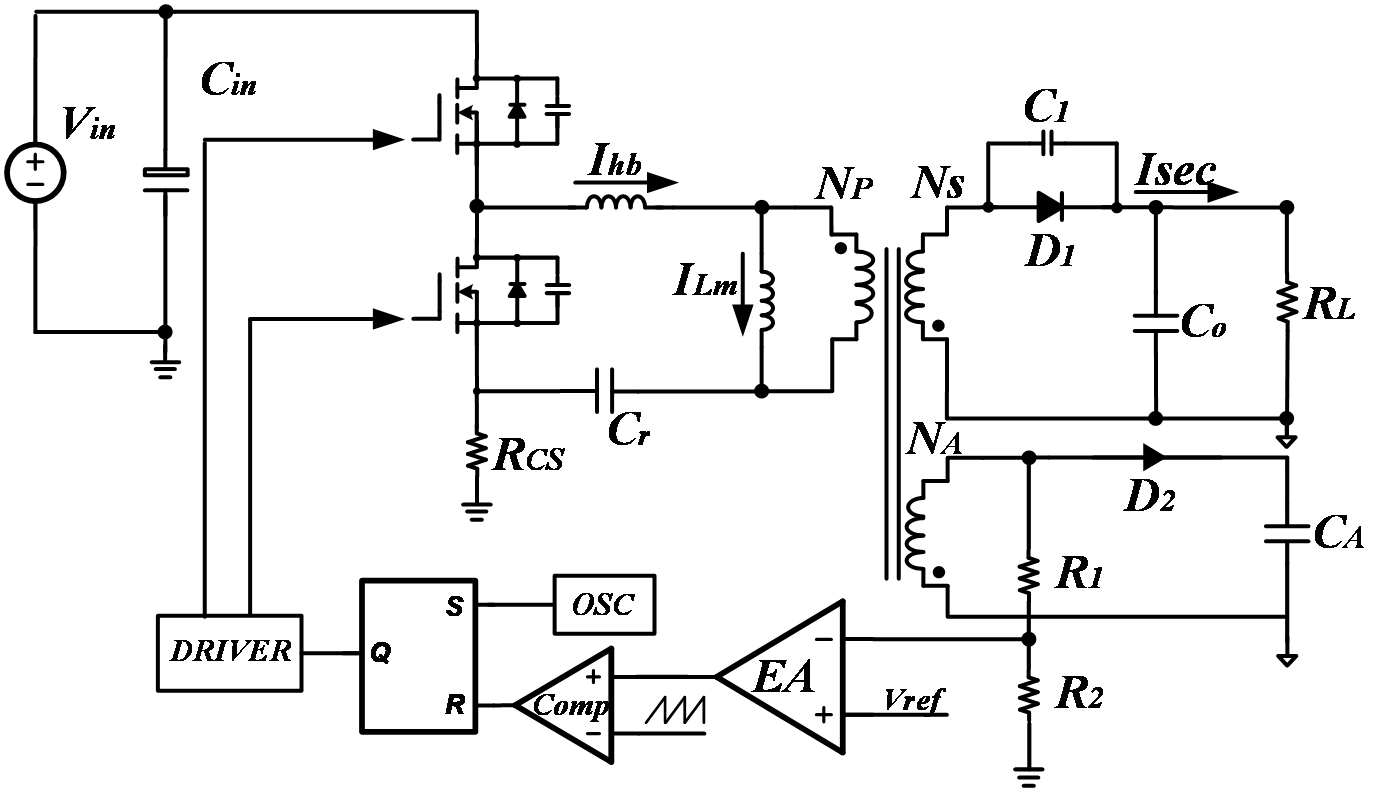
\includegraphics[width=0.8\linewidth]{figures/电压工作模式电路图.png}
    \caption{电压工作模式电路图}
    \label{fig:电压工作模式电路图}
\end{figure}

电压控制环路虽然结构简单且易于控制,但是由于只有一个电压环路,故只有当输出电压发生变化之后才会影响功率管的导通和关断时间,开始进行闭环负反馈动态调节,当输入电压产生干扰时,原边电感电流的上升斜率发生变化,会影响原边励磁电感的储能,但电压环路的控制和调节不会立即发生作用,而是在延迟一段时间之后才会起作用,系统整体的动态响应就会变差,输出电压产生很大的上冲和下冲现象。

\subsection{电流控制模式}

电流控制环路属于多环路控制方式,典型电路图如~\ref{fig:电流工作模式电路图}所示,包含一个电压环路和一个电流环路,电压环路和电压控制环路相同,采样输出电压信号用于生成误差放大信号;电流环路则是实时采样功率管的电流作为反馈电流,用采样电阻将电流转换为采样电压替代电压控制模式中的锯齿波信号,同误差放大信号VEA进行比较。

\begin{figure}[htbp] 
    \centering
    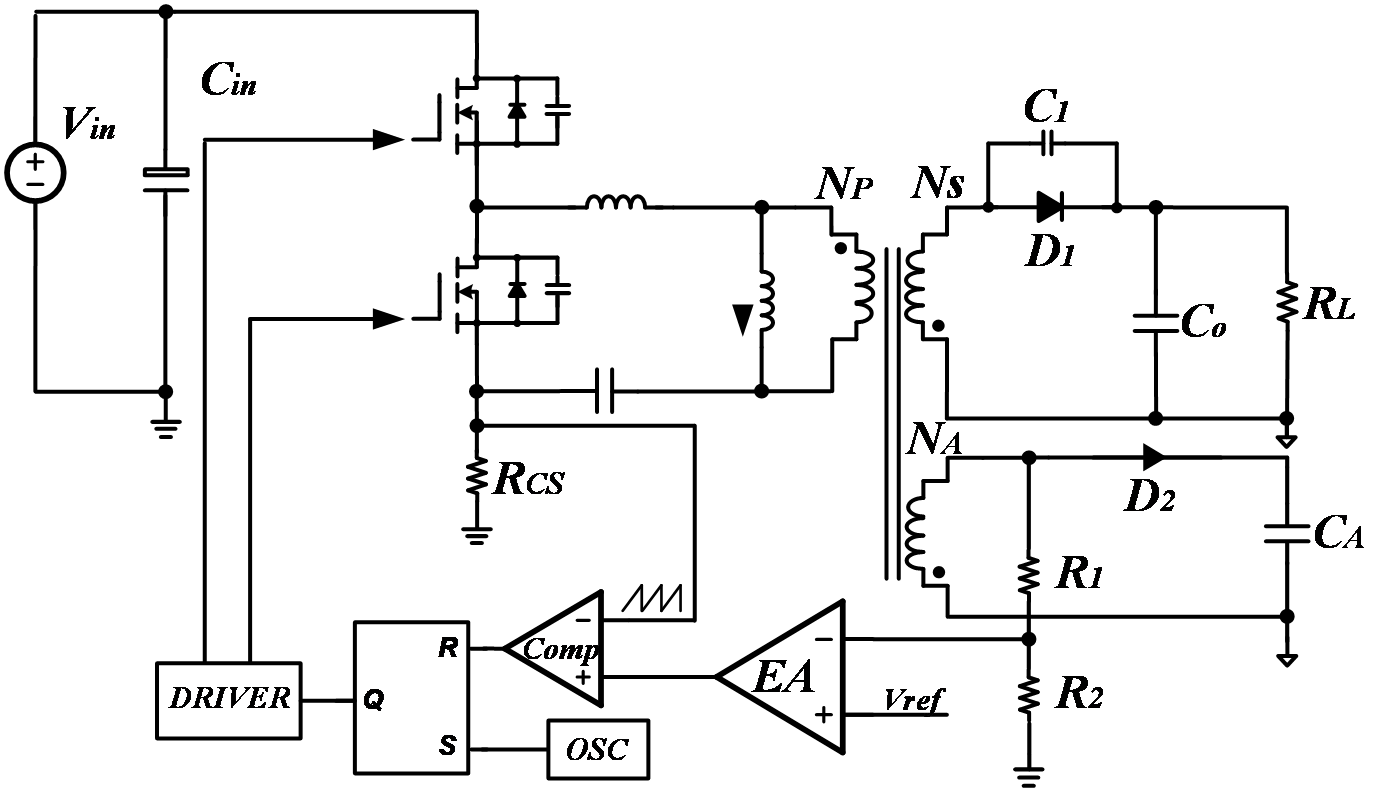
\includegraphics[width=0.8\linewidth]{figures/电流工作模式电路图.png}
    \caption{电流工作模式电路图}
    \label{fig:电流工作模式电路图}
\end{figure}

相比于电压控制模式对输入电压信号的不敏感,电流控制模式对输入输出信号都可以进行反馈,输入电压信号的变化会影响功率管导通时刻的电流斜率,通过采样电阻后产生一个随输入电压变化而变化的锯齿波信号,当输入电压发生扰动时,反馈环路可以直接响应改变功率管导通时间,而不需要等待输出电压信号发生相应波动后改变VEA的大小再影响功率管导通时间,极大地提高了系统整体的动态响应时间。但由于电流控制模式包含两个反馈环路,增大了电路结构的设计复杂度,另外,当驱动信号的占空比大于 50\%时,电路中不可避免地会出现次谐波振荡, 这需要增加额外的斜坡补偿电路来解决,一定程度上,也增加了应用难度。

 
\section{开关电源的反馈方式}
反激式开关电源变换器电路为保证输出电压稳定,进行闭环回路控制,需要对输出电压信号进行采样,并通过不同的方式将其反馈到变换器芯片进行逻辑处理。反激式开关电源变换器根据反馈结构的不同分为原边反馈(PSR)和副边反馈(SSR)两种反馈方式。其中原边反馈是通过辅助绕组对副边输出电压信号进行检测采样,副边反馈是通过 TL431 稳压模块和光耦模块组成的反馈系统对输出电压信号进行检测采样。

\subsection{原边反馈电路}
非对称半桥反激式变换器的原边反馈电路拓扑结构如~\ref{fig:原边反馈电路电路图}所示。

\begin{figure}[htbp] 
    \centering
    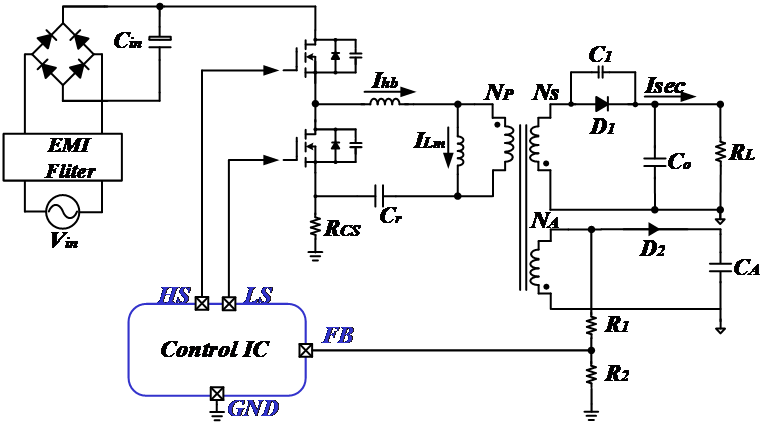
\includegraphics[width=0.8\linewidth]{figures/原边反馈电路图.png}
    \caption{原边反馈电路电路图}
    \label{fig:原边反馈电路电路图}
\end{figure}

原边反馈电路依靠辅助绕组采样输出电压,隔离变压器的特性是原边绕组、副边绕组和辅助绕组两端的电压相互成比例,原边绕组和辅助绕组电压极性相反,副边绕组和辅助绕组电压极性相同,因此辅助绕组电感电压值等于输出电压乘以副边绕组和辅助绕组的匝数比。在非对称半桥反激式开关电源系统中,在高边功率管导通阶段辅助绕组电感电压绝对值正比于原边绕组电感电压;低边功率管导通阶段辅助绕组检测副边绕组电感电压。辅助绕组电感电压VA经过R1和R2分压后得到原边反馈电压VFB送入变换器控制IC中参与闭环环路控制用以维持在负载变化情况下输出电压的稳定性。VA和VFB的电压值由式\eqref{eq:辅助绕组电压}和式\eqref{eq:VFB公式}所示:

\begin{equation}
    \label{eq:辅助绕组电压}
    V_A = \frac{N_A}{N_S}\times(V_O + V_{D1})
\end{equation}

\begin{equation}
    \label{eq:VFB公式}
    V_{FB} = V_A\times\frac{R_2}{R_1+R_2}=\frac{N_A}{N_S}\times(V_O + V_{D1})\times\frac{R_2}{R_1+R_2}
\end{equation}

\subsection{副边反馈电路}
非对称半桥反激式变换器的副边反馈电路拓扑结构如~\ref{fig:副边反馈电路电路图}所示。

\begin{figure}[htbp] 
    \centering
    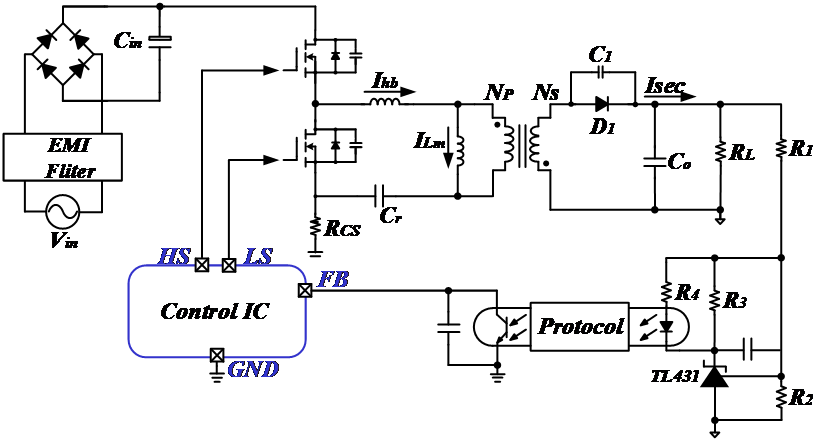
\includegraphics[width=0.8\linewidth]{figures/副边反馈电路图.png}
    \caption{副边反馈电路电路图}
    \label{fig:副边反馈电路电路图}
\end{figure}

副边反馈电路主要通过变压器副边侧基于TL431的反馈系统采集输出电压信号,该反馈系统包括输出电压分压电阻串R1和R2、TL431稳压模块、光电耦合器以及用于补偿的电容电阻。输出电压Vo通过分压电阻串R1和R2分压后送入TL431稳压模块中与其中自带的2.5V参考电压比较后产生一个误差信号,该误差信号经过光电耦合器,将电信号转化为光信号传输到变压器原边后再转化为电信号,实现变压器原副边电气隔离,TL431稳压模块可类似为一个误差放大器,通过额外的电阻电容组成的补偿网络对TL431输出的误差信号进行补偿,相当于集成在原边反馈系统变换器中的反馈网络移到了片外,可以根据不同的情况通过改变电阻电容的方式进行更精确的调节,将包含输出电压和负载电流信息的反馈电压VEA传递给变换器中。

相比于副边反馈电路,原边反馈电路由于不需要额外的外围电路,通过将反馈电压VFB输入变换器芯片内与参考电压在误差放大器中比较后输出误差放大信号Vea用于反馈环路的调节,具有较高的集成度,极大地节省了芯片外围电路板的面积,但由于副边绕组的电感电压并不完全等于输出电压,而是等于输出电压和副边续流二极管导通电压之和,导致副边绕组电感电压还可能受到负载电流和温度等因素的影响,且辅助绕组和副边绕组间存在的不匹配的情况,也将导致实际反馈电压值异于式(2-)的计算值,故而相比于副边反馈,原边反馈的采样准确性明显更低,为了消除这些误差,原边反馈电路需要添加更多的补偿电路极大增大电路设计复杂度,增大芯片的面积和功耗。因此副边反馈电路广泛应用于工业届,几乎所有的中等功率消费类电源都使用副边反馈系统。



 






















